\section{Mappatura sistema di illuminazione}
\label{sec:chapter_creazione_scena_mapping_illuminazione}
Nel paragrafo \ref{sec:chapter_baking_service_pipeline_baking_mapp_parametri} , si è discusso circa la realizzazione di una mappatura esplicita dei parametri tra ThreeJS e Blender. 
\\
Inoltre sono stati individuati quei parametri in grado di conferire alle SpotLight di ThreeJS delle caratteristiche, per quanto riguarda la luce diretta, simili a quelle della Spot Lamp di Blender. Si è parlato inoltre di come questi parametri vengano preconfigurati all’interno dell’Editor. In particolare, nel momento in cui l’utente clicca sull’opzione per inserimento di una SpotLight all’interno della scena, un nuovo oggetto di tipo \texttt{THREE.SpotLight} viene creato; prima dell’inserimento vengono preimpostati i parametri \texttt{distance} , \texttt{exponent}, e \texttt{decay} , come discusso in \ref{sec:chapter_baking_service_pipeline_baking_mapp_parametri} .
\\ 
L’adattamento delle SpotLight di ThreeJS alle Spot Lamp di Blender non si limita alle caratteristiche di irradiazione diretta, ma riguarda anche il modo in cui la sorgente luminosa può essere utilizzata all’interno della scena. 
\\
In particolare le SpotLight di ThreeJS, così come le DirectionalLight, nel momento in cui vengono aggiunte alla scena hanno un target fisso al centro di essa. Questo vuol dire che qualsiasi sia lo spostamento delle due sorgenti luminose, queste rimarranno orientate verso il centro della scena. Questa caratteristica potrebbe ridurre l’usabilità delle sorgenti luminose se si decidesse di orientarle in punti differenti.
\\ 
Ciò che avviene in Blender è che invece le SpotLamp, così come le Sun Lamp, inizialmente non sono ancorate a nulla; pertanto sono completamente orientabili in qualsiasi punto all’interno della scena. In caso poi l’utente decidesse di ancorare la luce ad un punto preciso, potrà farlo mediante apposità funzionalità.
\\
\begin{figure}[h]
 \centering
 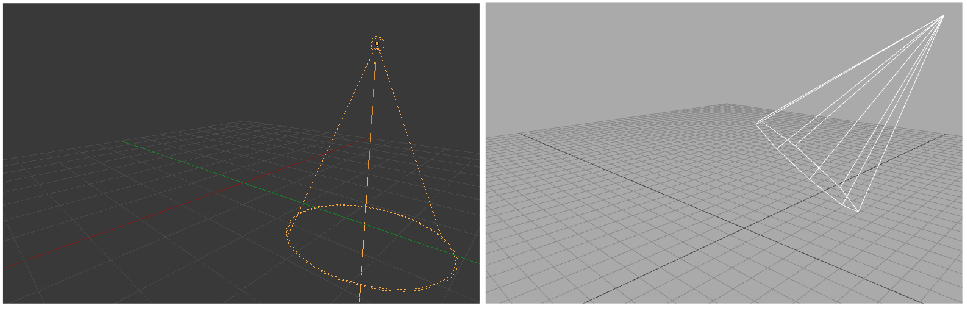
\includegraphics[width=1\linewidth]{images/chapter_creazione_scena/editor_5.png}\hfill
 \caption[Confronto luci]{Confronto tra una Spot Lamp standard generata in Blender, a sinistra, ed una SpotLight generata in una prima versione dell'editor, a destra. Si noti come nel primo caso, nonostante lo spostamento, la Spot Lamp con segua alcun target all'interno della scena, contrariamente a quanto a accade con la SpotLight, a sinistra, la quale rimane orientata verso il centro della scena.}
 \label{fig:editor_5}
\end{figure} 

Per adattare le luci di ThreeJS a quelle Blender è necessario quindi che il target originale, ossia quello fisso al centro della scena, venga modificato con un target mobile, che segua i movimenti della sorgente luminosa. L’oggetto rappresentante il nuovo target della SpotLight può essere un comune THREE.Object3D.
\\
Per far si che il nuovo target segua ogni movimento della sorgente luminosa, deve essere figlio della sorgente stessa. Una volta configurata la relazione gerarchica, è possibile associare all’attributo target della sorgente luminosa il nuovo Object3D creato. Per orientare l’irradiazione della luce verso il target è necessario che l’Object3D si trovi ad una certa distanza lungo la normale della sorgente.
\\
In questo modo sono stati concatenati due eventi:
\begin{itemize}
\item Al movimento della sorgente luminosa, il target di essa si muoverà con lei.
\item Al movimento del target, la sorgente luminosa manterrà il fascio orientato su di esso.
\end{itemize}
Di conseguenza la luce è tecnicamente ancorata ad un target fisso, in quanto il target condivide il sistema di riferimento del modello della sorgente luminosa, quindi rispetto ad essa l’oggetto target appare immobile. In verità nel sistema di riferimento in coordinate mondo entrambi si muovono insieme, come fossero un’unica entità. Ciò conferisce alla sorgente luminosa la possibilità di essere orientata in qualsiasi modo all’interno della scena, come avviene appunto per la configurazione standard delle sorgenti luminose in Blender.
\\
\begin{figure}[h]
 \centering
 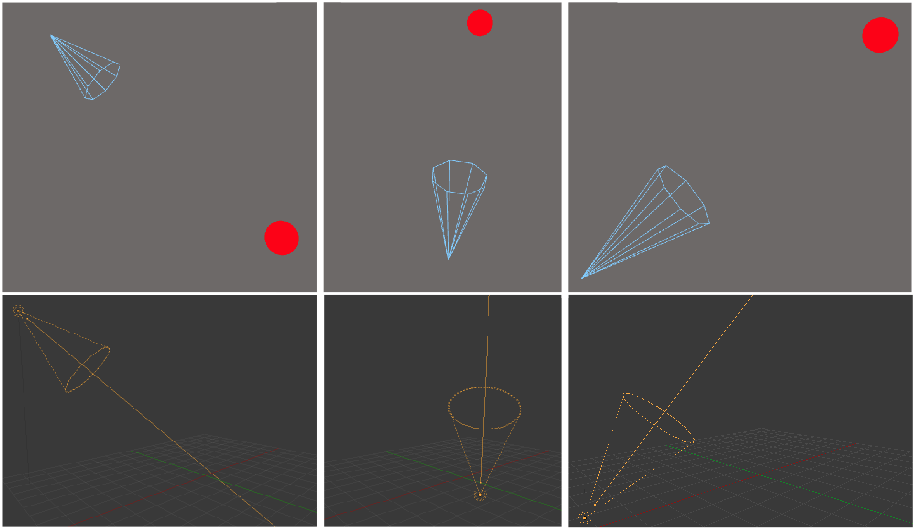
\includegraphics[width=1\linewidth]{images/chapter_creazione_scena/editor_6.png}\hfill
 \caption[Adattamento illuminazione]{In foto, il risultato dell'adattamento delle SpotLight di ThreeJS alle Spot Lamp di Blender. Notare come adesso sia possibile muovere le luci nello stesso modo, grazie al doppio legame tra la SpotLight e il rispettivo target (la sfera rossa in ogni foto della sequenza in alto).}
 \label{fig:editor_6}
\end{figure} 

La procedura sopra descritta ha permesso di adattare il fascio di irradiazione delle sorgenti luminose, ma siccome ogni luce in ThreeJS è composta anche da un’oggetto \texttt{Helper} della luce, ossia un wireframe che serve ad individuare posizione ed orientamento del fascio luminoso nello spazio, si è reso necessario risolvere alcuni problemi di ThreeJS legati all’orientamento degli helper delle SpotLight e delle DirectionalLight.
\\ 
In particolare adattando una luce con il metodo sopra esposto, il relativo helper non seguiva appieno i movimenti del fascio luminoso.
\\
Per risolvere questo problema è stato necessario apportare delle modifiche all’interno delle classi \texttt{THREE.SpotLightHelper} e \texttt{THREE.DirectionalLightHelper} , in particolare nel metodo \texttt{update()} di entrambe, il quale si occupa di aggiornare posizione e orientamento dell’Helper nello spazio della scena.
\\
Entrambi i metodi update sono stati semplificati, specificando solamente che il valore dell’attributo \texttt{lootAt} dell’oggetto rappresentante l’Helper, che nel caso della SpotLight è il wireframe di una geometria conica, ad ogni invocazione del metodo update() deve essere aggiornato con la posizione corrente del target. 